\documentclass{article}

\usepackage[T1]{fontenc}
\usepackage{microtype}
\usepackage{graphicx}
\usepackage{booktabs}
\usepackage{amsmath}
\usepackage{amssymb}
\usepackage{hyperref}
\setlength{\emergencystretch}{2em}

\newcommand{\theHalgorithm}{\arabic{algorithm}}

\usepackage[accepted]{mlsys2025}

\makeatletter
\renewcommand{\mlsys@appearing}{Copyright 2026 by the author.}
\renewcommand{\Notice@String}{\mlsys@appearing}
\makeatother

\hypersetup{
  pdftitle={What Training Data Should Carry: Local Fine-Tuning, Loss Masking, and the Retrieval That Beats It},
  pdfauthor={Gege Ardiyansyah},
  pdfsubject={Systems for Machine Learning}
}

\mlsystitlerunning{What Training Data Should Carry: Local Fine-Tuning and Loss Masking}

\begin{document}

\twocolumn[
\mlsystitle{What Training Data Should Carry: Local Fine-Tuning, Loss Masking, and the Retrieval That Beats It}

\begin{mlsysauthorlist}
\textbf{Gege Ardiyansyah}
\end{mlsysauthorlist}

\mlsystitlerunning{What Training Data Should Carry: Local Fine-Tuning and Loss Masking}
\mlsyskeywords{local fine-tuning, LoRA, PII sanitization, canary exposure, Graph-PPR, Cache-Augmented Generation, compliance QA}

\vskip 0.3in

\begin{abstract}
Organizations frequently seek to adapt small open-weight language models to internal regulatory corpora without transmitting raw source documents to external cloud services. This paper asks what the resulting training data should carry, and answers it in three parts on a single 8\,GB RTX~4070 Laptop GPU across three fine-tuned models (\texttt{Qwen2.5-0.5B-Instruct}, size-matched \texttt{Qwen2.5-1.5B-Instruct}, and \texttt{LFM3-1.7B-Base}) plus three quantized Ollama inference comparators. First, redaction is necessary: with matched raw-versus-redacted chat SFT pairs, raw \texttt{T2-Chat} LoRA memorizes $20\times$-repeated Carlini canaries into weights ($8.25$--$8.40$ bits, up to $6/12$ Rank-1) and leaks $11/12$ secret spans verbatim at prompt time on \texttt{qwen2.5:7b}, whereas local PII redaction cuts canary exposure to $2.63$--$3.51$ bits (including $0/12$ Rank-1 on \texttt{Qwen2.5-1.5B}) and removes verbatim adversarial context extraction ($11/12 \to 0/12$) at $0.0\%$ compliance QA accuracy loss. Second, when fine-tuning on redacted text is the chosen path, it inherits a distinct failure mode that we call \emph{placeholder-token gradient domination}: standard cross-entropy SFT over targets containing \texttt{<PII:...>} placeholders yields $40\%$--$85\%$ tag hallucination on seen documents and $20\%$--$47.5\%$ in-scope false refusals under the \texttt{Safe} arm, and we describe an operational account in which the adapter is dominated by high-surprisal placeholder tokens rather than by the intended content. Privacy-Token Loss Masking (\texttt{PT-LM}), which masks placeholder subwords from the backward loss and substitutes grammatical-role surrogates in the forward context, reduces tag emission to $0.0\%$ ($0$ of $210$, three models $\times$ $70$ questions) and in-scope false refusals to $0.0\%$, lifting seen-document F1 on all three models ($+0.194$, $+0.087$, $+0.117$; $p = 0.0005$ and $0.001$ on the Qwen models, $p = 0.083$ and not significant on \texttt{LFM3-1.7B}) and held-out in-scope blinded judge scores on every model. An $18$-adapter step and learning-rate grid confirms the protection is recipe-robust: no adapter exceeds its base exposure, with the smallest margin $0.03$ bits (\texttt{LFM3-1.7B}, $80$ steps, $1\mathrm{e}{-4}$) reported without an interval. A fourth, explicitly exploratory arm (\texttt{IB-PT-LM}) adds a $\beta{=}0.2$ symmetric-KL term between two disjoint surrogate pools on one \texttt{0.5B} model and cuts suffix-inversion exposure from $5.27$ to $1.15$ bits and an $8$-way hidden-state probe from $37.50\%$ to $19.79\%$ at $\approx 2.05\times$ training cost. Third, and despite this repair, zero-training retrieval remains the stronger default at this scale: Dual-CSR Graph-PPR (\texttt{versieve\_graph.wasm}) outperforms every closed-book LoRA arm, including \texttt{PT-LM}, on held-out compliance QA across both blinded \texttt{qwen2.5:7b} and cross-family \texttt{llama3.2:3b} judges ($p = 0.0005$ on F1), at lower latency. PT-LM's niche is therefore the case where weight-held redacted fine-tuning is required for reasons outside QA: offline or re-indexing-free deployment.
\end{abstract}
]

\section{Introduction}
\label{sec:intro}

Adapting language models to an organization's own compliance and policy documentation can improve domain grounding, but uploading sensitive source records to a hosted fine-tuning API introduces unacceptable data-egress risk. A natural alternative is to extract, deduplicate, and sanitize documents entirely on local hardware, then perform either local parameter-efficient fine-tuning or local retrieval strictly over the sanitized artifacts.

This paper benchmarks three practical questions that determine how local compliance systems should be built on consumer GPU hardware:
\begin{enumerate}
    \item \textbf{Does local data redaction matter for open-weight models?} When identical compliance excerpts and planted secrets are processed in matched raw versus PII-redacted arms across both Transformer (\texttt{Qwen2.5}) and hybrid (\texttt{LFM3}) architectures, how strongly does local sanitization prevent weight-level canary memorization and prompt-time context extraction, and what utility cost does it impose?
    \item \textbf{When fine-tuning on redacted text is the chosen path, can the placeholder-token failure mode be removed at the loss level?} Under assistant-only chat SFT on redacted targets (\texttt{T2-Chat}), small models hallucinate \texttt{<PII:...>} placeholder tags and falsely refuse in-scope questions; we test whether Privacy-Token Loss Masking (\texttt{PT-LM}) removes both failure modes and what it changes.
    \item \textbf{Can fine-tuned local LoRA beat zero-training retrieval?} With the above resolved, does local LoRA fine-tuning outperform zero-training WebAssembly Graph-PPR retrieval or KV-cached Native CAG on held-out or even \emph{in-training} compliance documents?
\end{enumerate}

The paper additionally reports an explicitly exploratory counterfactual information-bottleneck arm (\texttt{IB-PT-LM}, Section~\ref{sec:ib-ptlm}), a surrogate-invariance sharpener for \texttt{PT-LM} on one \texttt{0.5B} model; it is a pilot, not a headline contribution.

The extraction, redaction, and retrieval pipeline itself is specified and evaluated in the companion paper on local extraction, redaction, and fail-closed gatekeeping \citep{ardiyansyah2026extraction}; this paper is the full study of what that pipeline means for local fine-tuning.

We evaluate these questions across three locally fine-tuned models (\texttt{Qwen2.5-0.5B-Instruct}, size-matched \texttt{Qwen2.5-1.5B-Instruct}, and \texttt{LFM3-1.7B-Base}) and three quantized Ollama inference comparators (\texttt{lfm3:latest}, \texttt{llama3.2:3b}, and \texttt{qwen2.5:7b}) \citep{liquidai_lfm3_base,liquidai_lfm3_chat}. Figure~\ref{fig:training-arch} illustrates the end-to-end local corpus split, sanitization, parallel adaptation/retrieval paths, and privacy verification harness.

\begin{figure*}[t]
\centering
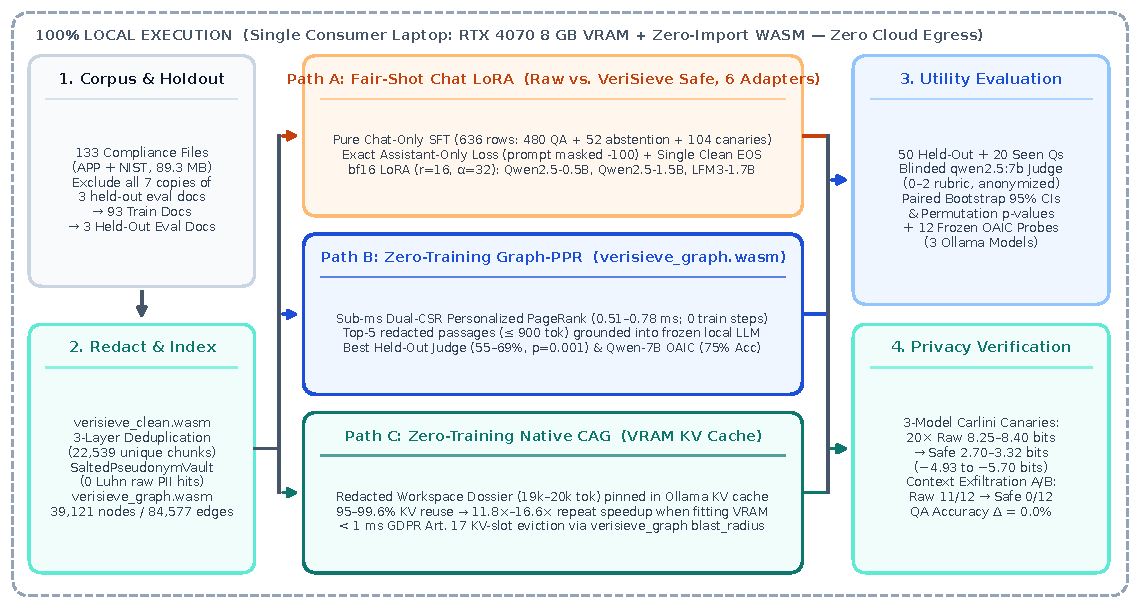
\includegraphics[width=0.98\textwidth]{figs/fig1-training-architecture.pdf}
\caption{End-to-end local training, retrieval, and privacy-verification architecture on an 8\,GB RTX~4070 Laptop GPU. After excluding all $7$ copies of the $3$ held-out evaluation documents, the remaining compliance files are deduplicated (\texttt{versieve\_clean.wasm}), redacted (\texttt{SaltedPseudonymVault}), and indexed (\texttt{versieve\_graph.wasm}), then evaluated in parallel across matched Raw vs.\ Safe assistant-only-loss Chat LoRA adapters (Path~A), zero-training Graph-PPR retrieval (Path~B), and zero-training Native CAG with sub-millisecond GDPR Art.~17 KV-slot eviction (Path~C).}
\label{fig:training-arch}
\end{figure*}

\section{Related Work and Scope}
\label{sec:related}

The core building blocks of our benchmark are well established: Low-Rank Adaptation (LoRA) updates frozen language models using compact rank-decomposed matrices \citep{hu_lora}; canary exposure quantifies unintended secret memorization during training \citep{carlini_secret_sharer}; and PrivacyQA benchmarks question answering over privacy policies \citep{ravichander_privacyqa}. Prior privacy analyses show that text scrubbing reduces but does not fully remove PII leakage in fine-tuned models \citep{lukas_pii_leakage}, that frontier language models can infer private attributes from scrubbed text despite anonymization \citep{staab2024beyond}, and that LoRA adapters can retain planted secrets depending on adapter placement and repetition \citep{tan_lora_memorization}. Person-identity deletion under sanctioned erasure requests is, separately, an active 2026 benchmark axis in the unlearning literature: PRMU studies corpus-free person-centric knowledge unlearning in multimodal large language models under realistic person deletion requests, with naturally acquired person knowledge and a locality analysis \citep{prmu2026person}, alongside AIM \citep{aim2026person}, PPU-Bench \citep{ppubench2026}, and UnPII \citep{unpii2026}, all unrefereed preprints. That line evaluates model-parameter unlearning under deletion requests, whereas this paper measures pre-training redaction effects on canary exposure and prompt-time extraction and makes no unlearning claim; and canary thresholds themselves are model-dependent, since the repetition count before planted email and phone strings become extractable is reported to vary substantially across four models in a $1\times$ to $50\times$ sweep \citep{fcpa2026cana}, consistent with the per-model exposure differences measured here on the three tested models.

Selective token loss masking and type-consistent surrogate substitution both have direct prior art. Selective cross-entropy masking over tokens appears in data-efficiency pretraining (\texttt{Rho-1} \citep{lin2024rho1}), memorization mitigation (\texttt{Goldfish Loss} \citep{hans2024goldfish}), and privacy-focused fine-tuning (\texttt{SLUNG} \citep{wang2025slung}, \texttt{RMFT} \citep{joshi2025rmft}, and \texttt{Surprise Masking} \citep{tyagi2026surprise}), while local type-consistent surrogate substitution is studied end-to-end for privacy, utility, and LoRA trainability in \texttt{Anonymous-by-Construction} \citep{albanese2026anonymous}. Accordingly, our \texttt{PT-LM} claim is narrowed specifically to mitigating placeholder-token tag echo and in-scope false refusal on small $0.5\text{B}$--$1.7\text{B}$ LoRA adapters via the bundled $-100$ placeholder loss mask, grammatical-role forward surrogates, and scope-balanced abstention subsampling, rather than claiming general mechanism novelty for token loss masking or surrogate substitution; Section~\ref{sec:ptlm-r4} separates the three across three seeds.

The exploratory \texttt{IB-PT-LM} arm (Section~\ref{sec:design}) sits in a literature whose every component has prior art. The information bottleneck frames representation learning as compression while preserving the target \citep{tishby2015ib}, and variational IB objectives train stochastic encoders under an IB penalty \citep{alemi2017vib}; counterfactually augmented data rewrites only a sensitive attribute to teach invariance \citep{kaushik2020counterfactual}; IRM-style objectives penalize predictors that move across environments \citep{arjovsky2019irm}; and symmetric KL between teacher or peer logits underlies distillation and co-distillation \citep{hinton2015distilling,anil2018online}. The delta claimed here is narrow: two strictly disjoint surrogate pools plus an aligned, non-PII-token-restricted symmetric KL term as a training-time invariance objective over redaction surrogates; the combination, not any component, is the contribution.

Our zero-training-versus-fine-tuning comparison therefore positions as replication with amplification: it extends the known finding that retrieval outperforms fine-tuning for knowledge injection \citep{ovadia2023finetuning} and that parametric memory is weakest exactly where compliance corpora live, on long-tail facts \citep{mallen2023when,kandpal2023longtail}, to a 0.5B--1.7B envelope on one 8\,GB consumer GPU, with a privacy twist that prior work in this line does not carry: the fine-tuning data itself is redacted rather than raw. Contemporaneous funded-scale work reports the crossover in the other direction once the data pipeline and the budget grow: MeMo \citep{quek2026memo} fine-tunes a dedicated Memory model on a generator-driven five-step curated QA pipeline and reports a frozen Executive LLM querying the trained weights outperforming HippoRAG2, NV-Embed-V2, and BM25 on two of three multi-hop benchmarks (NarrativeQA and MuSiQue) with a $14$B Memory model, while narrowly trailing HippoRAG2 on BrowseComp-Plus under one of its two Executives. Its $1$--$2$B ablation models (Qwen2.5-1.5B, Gemma3-1B, and LFM2.5-1.2B) sit inside our scale envelope; we run no head-to-head against it. MeMo remains a non-peer-reviewed preprint (May 2026, venue status marked), carries no PII, memorization, or erasure analysis, and its own impact statement notes that the approach may obscure the provenance of retrieved information and that each new corpus incurs an upfront retraining cost; the deterministic byte-verified regeneration and sealed retrain recipe of the companion corpus paper \citep{ardiyansyah2026graphcorpus} are the compliance half that design leaves missing. Our contribution relative to these results is the controlled, zero-egress local systems benchmark spanning portable PDF/OCR extraction, format-validated regex and salted-pseudonym masking, matched raw-versus-sanitized chat LoRA training with exact assistant-only loss across three models (0.5B, 1.5B, and 1.7B), blinded local LLM-as-a-Judge grading with paired bootstrap confidence intervals, and direct comparison against sub-millisecond WebAssembly Graph-PPR and KV-cached Native CAG. We do not claim formal differential privacy guarantees, neural NER parity, or expert legal certification.

\section{System Pipeline and Corpus Construction}
\label{sec:corpus}

All document ingestion ran locally using Versieve's portable extraction core and zero-import WebAssembly kernels (\texttt{versieve\_clean.wasm} and \texttt{versieve\_graph.wasm}), without cloud APIs. The gatekeeper itself, including its multimodal fail-closed path, is specified and evaluated in the companion multimodal-sanitization paper \citep{ardiyansyah2026multimodal}; this paper uses it only as a stage. The initial $83$-file extraction ($52$ PDFs, $30$ PNGs, $1$ mislabeled HTML file) yielded $180{,}411$ candidate lines routed by the local gatekeeper (Table~\ref{tab:extraction}); PNG OCR produced $2{,}090$ lines and zero \texttt{KEEP\_SAFE} rows.

\begin{table}[t]
\caption{Gatekeeper routing distribution across the initial $83$-file extraction (\texttt{T1} corpus baseline).}
\label{tab:extraction}
\vskip 0.08in
\begin{center}
\begin{tabular}{lrr}
\toprule
\textbf{Gatekeeper Action} & \textbf{Lines} & \textbf{Share} \\
\midrule
\texttt{KEEP\_SAFE} & $100{,}463$ & $55.7\%$ \\
\texttt{DROP\_OR\_QUARANTINE} & $20{,}033$ & $11.1\%$ \\
\texttt{ABSTAIN\_HUMAN\_REVIEW} & $59{,}915$ & $33.2\%$ \\
\midrule
\textbf{Total} & $\mathbf{180{,}411}$ & $\mathbf{100.0\%}$ \\
\bottomrule
\end{tabular}
\end{center}
\vskip -0.14in
\end{table}

In the expanded $133$-file ($89.3$\,MB) compliance repository (\texttt{APP} and \texttt{NIST}), we removed legacy URL auto-drop rules, allowed cleanly redacted prose to pass as safe, and applied three-layer deduplication (file SHA-256, chunk exact SHA-256 plus $64$-lane MinHash at $0.85$ Jaccard, and output record SHA-256). Across $101$ supported files ($1$ exact duplicate skipped), this removed $4{,}188$ boilerplate chunks, $3{,}999$ exact duplicate chunks, and $3{,}346$ near-duplicate chunks, yielding $22{,}539$ unique chunks indexed into $39{,}121$ graph nodes and $84{,}577$ edges in $40.7$\,s.

\section{Experimental Design}
\label{sec:design}

\subsection{Strict Holdout Split and Seen-Document Recall Probe}
Three complete regulatory documents underpin our $50$-question held-out benchmark ($40$ in-scope, $10$ out-of-scope): the NIST AI Risk Management Framework (AI~100-1), OAIC Australian Privacy Principles Chapter~1, and the Privacy Act 1988 compilation \citep{nist_ai_rmf,oaic_app_guidelines,privacy_act_1988}. All $7$ file copies matching these three documents were excluded prior to indexing and training. To ensure closed-book LoRA is also evaluated on material it actually saw during training, we additionally construct a $20$-question \emph{seen-document} factual recall probe (\texttt{seen\_20q}) using paraphrased questions grounded across $20$ distinct in-training compliance documents.

\subsection{Training Regimes: Flat \texttt{T1}, Fair-Shot \texttt{T2-Chat}, and Privacy-Token Loss Masking (\texttt{PT-LM})}
\begin{itemize}
    \item \textbf{Flat-Line Baseline (\texttt{T1}):} $1{,}500$ short excerpts ($49.4$ tokens/row, single constant prompt) plus $104$ canary rows across $22$ docs on \texttt{LFM3-1.7B-Base} ($401$ steps, $r=8, \alpha=16$). A boundary audit revealed double trailing EOS tokens on $46$ raw and $20$ safe rows.
    \item \textbf{Fair-Shot Pure Chat-Only LoRA (\texttt{T2-Chat}):} To remove both flat-line EOS collapse and raw-passage header imitation, we build strictly matched Raw and Versieve-Safe pure chat datasets ($636$ identical rows per arm across $89$ disjoint training docs: $480$ diverse compliance Q\&A turns, $52$ explicit out-of-scope abstention turns, and $104$ Carlini canary turns at $1\times$, $5\times$, and $20\times$; $0$ raw \texttt{packed\_passage} rows, $0$ raw canary leaks in Safe). Every adapter trains with \emph{exact assistant-only loss masking} (prompt tokens masked to $-100$, single clean EOS, \texttt{pad\_token\_id} $\neq$ \texttt{eos\_token\_id}), \texttt{bf16}, gradient checkpointing, $r=16$, $\alpha=32$, learning rate $2\mathrm{e}{-4}$, cosine schedule, batch size $2{\times}4$ (per-device $2$ with gradient accumulation $4$), max sequence length $768$, and $80$ optimizer steps across all architectures. Fair-shot here means a matched compute and recipe budget across the Raw, Safe, and \texttt{PT-LM} arms, not matched information access: the $636$ training rows carry a small fraction of the $22{,}539$ indexed chunks that the retrieval arm sees at inference.
    \item \textbf{Placeholder-Token Gradient Domination and Privacy-Token Loss Masking (\texttt{T2-Chat PT-LM}):} When a small language model ($0.5\text{B}$--$1.7\text{B}$) is fine-tuned with standard cross-entropy loss over redacted assistant targets containing synthetic placeholder tokens $\mathcal{P} = \{\texttt{<PII:PERSON\_k>}, \texttt{<PII:ADDRESS\_k>}, \dots\}$, those out-of-distribution bracket strings have near-zero prior probability under the pretrained base model ($p_{\theta_0}(y_t \in \mathcal{P} \mid y_{<t}) \ll 10^{-5}$). Consequently the rank-$r$ LoRA update gradient $\nabla_{\Delta W}\mathcal{L}_{\text{CE}}$ is weighted toward the high-surprisal $\mathcal{P}$ tokens, and the fine-tuned model spontaneously emits \texttt{<PII:...>} tags during open-ended compliance QA ($65.0\%$, $13/20$, of seen-document answers under \texttt{T2-Chat Safe}). We name this failure mode \textbf{placeholder-token gradient domination}.
 The name is operational: gradient allocation into the placeholder subspace was not measured directly, and a surface-format imitation account, in which the adapter copies a frequent literal string present in the targets, predicts the same tag echoes and is removed by the same fix. No measured mechanism is claimed. To remove this failure mode at the loss level, Versieve's \texttt{perceive()} tokenizer (\texttt{computePtlmMaskedSpans}) implements \textbf{Privacy-Token Loss Masking (\texttt{PT-LM})}:
    \begin{equation}
      \mathcal{L}_{\text{PT-LM}}(\theta) = -\sum_{t \in \mathcal{T}_{\text{asst}} \setminus \mathcal{T}_{\mathcal{P}}} \log p_{\theta}\!\left(y_t \mid x,\; \tilde{y}_{<t}\right),
    \end{equation}
    where all subword indices $t \in \mathcal{T}_{\mathcal{P}}$ belonging to redacted placeholder spans are masked in the backward loss tensor ($\texttt{labels}[t] = -100$) and mapped in the forward context $\tilde{y}_{<t}$ to natural grammatical role surrogates $g(\text{type})$ (e.g., \textit{``the designated individual''}) while retaining zero raw PII in $\texttt{input\_ids}$. The abstention turns are the same $10\%$ explicit abstention turns already present in both \texttt{T2-Chat} arms. The mask covers $5.72\%$--$5.78\%$ of assistant target subwords ($2{,}655$ per arm). Because $\partial \mathcal{L}_{\text{PT-LM}} / \partial z_{t, v} = 0$ for all $t \in \mathcal{T}_{\mathcal{P}}$, the adapter receives zero gradient pressure to emit \texttt{<PII:...>} tags while preserving identical Carlini canary protection.
\item \textbf{Counterfactual Surrogate Information-Bottleneck LoRA (\texttt{IB-PT-LM}, exploratory):} Static \texttt{PT-LM} substitutes one fixed surrogate into the forward context, which the adapter can learn to condition on. \texttt{IB-PT-LM} trains two counterfactual views of every redacted row, drawing each view's surrogate from two strictly disjoint type-consistent pools, and adds a position-aligned symmetric KL over causal positions whose target is a non-PII token (placeholder positions are excused, so the KL never re-introduces pressure to emit tags), $\beta{=}0.2$:
    \begin{equation}
      \resizebox{\linewidth}{!}{$\displaystyle
      \mathcal{L}_{\text{IB-PT-LM}}(\theta) = \mathcal{L}_{\text{PT-LM}}(\theta) + \tfrac{\beta}{2}\Big(\mathrm{KL}(p^{A}_\theta \| p^{B}_\theta) + \mathrm{KL}(p^{B}_\theta \| p^{A}_\theta)\Big)_{\mathcal{T}_{\text{non-PII}}}$}
    \end{equation}
    where $p^{A}_\theta$ and $p^{B}_\theta$ are the next-token distributions of the pool-A and pool-B views. Pool disjointness is audited and checked in ($0$ shared strings per surrogate category), and is load-bearing: a shared pool would let the model collapse both views to the same surface strings and the KL would degenerate to zero.
\end{itemize}

\subsection{Dual Blinded Judges (\texttt{qwen2.5:7b} and Cross-Family \texttt{llama3.2:3b}), Statistical Tests, and Privacy Probes}
All inference ran locally on an NVIDIA GeForce RTX~4070 Laptop GPU ($8$\,GB VRAM, PyTorch~2.10.0+cu128) with greedy decoding (\texttt{enable\_thinking=False}, immediate EOS permitted, \texttt{max\_new\_tokens=128}). Beyond lexical token F1, key-point recall, empty-response rate, \texttt{<PII:...>} tag echo rate, in-scope false refusal rate, and out-of-scope abstention, every response across all conditions and $70$ questions was shuffled, stripped of arm identity, and graded on a $0$--$2$ rubric by a blinded local \texttt{qwen2.5:7b} LLM judge. To rule out same-family judge preference bias (position, verbosity, self-enhancement, and own-generation bias are documented failure modes of LLM judges \citep{zheng2023judging,wang2024fair,panickssery2024llm}), we additionally grade the key comparison arms (\texttt{T2-Chat Safe}, \texttt{T2-Chat PT-LM}, and \texttt{T0+Graph-PPR}) across all three models with an independent cross-family blinded local \texttt{llama3.2:3b} judge. We report $1{,}000$-resample paired bootstrap $95\%$ confidence intervals and $2{,}000$-resample two-sided paired permutation $p$-values, both paired over the shared question set. The permutation $p$-values are reported uncorrected, and the blinded judge-score summary cells are reported without an interval.

\paragraph{Artifact availability.} Every table in this paper is emitted by a checked-in runner in \url{https://github.com/gegearsyah/versieve} at commit \texttt{1e35603}; the main-suite training runner fixes the seed at 42 while the mechanism ablation (Section~\ref{sec:ptlm-r4}) runs seeds 42, 43, and 44, and the recipe-grid sweep JSON, multi-seed ablation JSON, and adapter metadata are included with the submission.

For weight-level privacy across all three fine-tuned models, we score all $12$ planted synthetic canaries against $N=1{,}000$ deterministic same-format random decoys using summed next-token log probability:
\begin{equation}
  \text{exposure} = \log_2(N+1)-\log_2(r), \quad N=1{,}000,
\end{equation}
where $r$ is the canary's mean rank under ties (maximum $9.97$ bits) \citep{carlini_secret_sharer}. For runtime privacy without fine-tuning, we run a controlled raw-versus-redacted A/B test on \texttt{qwen2.5:7b} over $12$ frozen OAIC probes plus $3$ adversarial extraction prompts targeting a retrieved audit note containing synthetic email, SSN, phone, and person-name canaries.

\section{Results}
\label{sec:results}

\begin{figure*}[t]
\centering
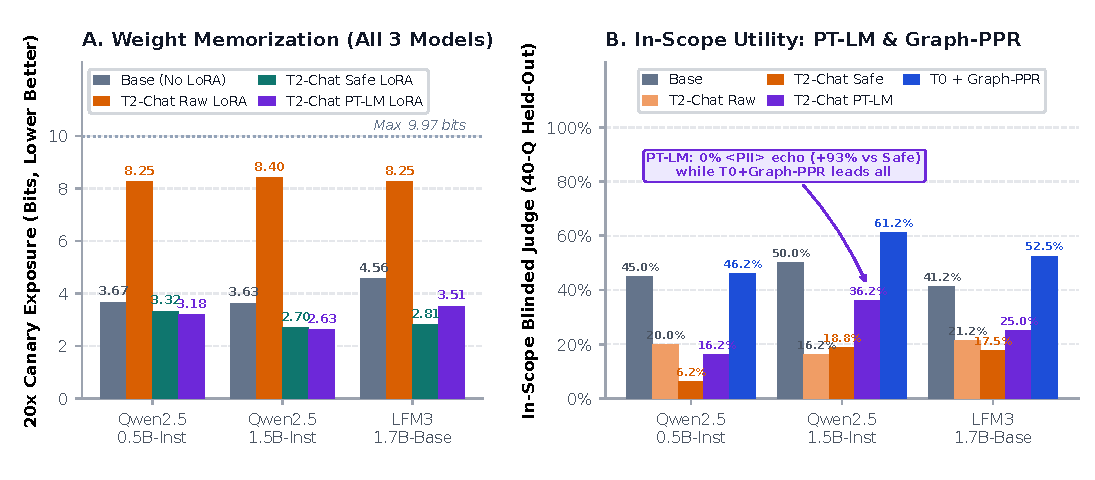
\includegraphics[width=0.98\textwidth]{figs/fig2-track-d-results.pdf}
\caption{Three-model fair-shot evaluation on an 8\,GB RTX~4070 Laptop GPU. \textbf{Panel A:} Carlini $20\times$-canary weight exposure spikes to $8.25$--$8.40$ bits under Raw Chat LoRA across all three models, whereas both Versieve \texttt{T2-Chat Safe} ($2.70$--$3.32$ bits) and \texttt{T2-Chat PT-LM} ($2.63$--$3.51$ bits) neutralize memorization back to or below the untrained base model. \textbf{Panel B:} In-scope blinded local \texttt{qwen2.5:7b} LLM-as-a-Judge scores across the $40$ in-scope held-out compliance questions show \texttt{T2-Chat PT-LM} removing \texttt{<PII:...>} tag hallucination ($0.0\%$) and lifting \texttt{T2-Chat Safe} utility by $+43\%$ to $+161\%$ ($6.2\% \to 16.2\%$, $18.8\% \to 36.2\%$, $17.5\% \to 25.0\%$), while zero-training \texttt{T0+Graph-PPR} ($46.2\%$, $61.2\%$, $52.5\%$) leads all closed-book LoRA arms across every model ($p = 0.0005$ on F1).}
\label{fig:trackd-results}
\end{figure*}

\subsection{Cross-Family Carlini Weight Exposure (All Three Models)}
The flat-line \texttt{T1} baseline motivates the chat-only design. In it, \texttt{LFM3-1.7B-Base} showed $90\%$--$92\%$ immediate-EOS collapse ($45$--$46/50$ empty responses), and Raw \texttt{T1} raised $20\times$-canary exposure from the untrained $4.45$ to $8.54$ bits ($5/12$ Rank-1) against $1.58$ bits ($0/12$ Rank-1) under Safe \texttt{T1}. Table~\ref{tab:canary} and Figure~\ref{fig:trackd-results} (Panel~A) show that this memorization-versus-protection dynamic replicates across all three models under the assistant-only \texttt{T2-Chat Safe} and \texttt{T2-Chat PT-LM} arms.

\begin{table*}[t]
\caption{Cross-family Carlini Secret-Sharer canary exposure (bits, max $9.97$) across $12$ synthetic canaries ($1\times$, $5\times$, $20\times$ repetitions) under matched fair-shot \texttt{T2-Chat} LoRA (Raw, Safe, and Privacy-Token Loss Masking \texttt{PT-LM}) on all three architectures.}
\label{tab:canary}
\vskip 0.08in
\begin{center}
\footnotesize
\setlength{\tabcolsep}{3.8pt}
\begin{tabular}{lrrrrrrrrrrrr}
\toprule
\textbf{Model} & \multicolumn{4}{c}{\textbf{All 12 Canaries (Bits)}} & \multicolumn{4}{c}{\textbf{20$\times$ Repetitions (4)}} & \multicolumn{4}{c}{\textbf{Rank-1 Memorized}} \\
\cmidrule(lr){2-5}\cmidrule(lr){6-9}\cmidrule(lr){10-13}
 & Base & Raw & \textbf{Safe} & \textbf{PT-LM} & Base & Raw & \textbf{Safe} & \textbf{PT-LM} & Base & Raw & \textbf{Safe} & \textbf{PT-LM} \\
\midrule
\texttt{Qwen2.5-0.5B-Instruct} & $3.84$ & $6.71$ & $\mathbf{3.45}$ & $3.68$ & $3.67$ & $8.25$ & $3.32$ & $\mathbf{3.18}$ & $1/12$ & $3/12$ & $\mathbf{1/12}$ & $\mathbf{1/12}$ \\
\texttt{Qwen2.5-1.5B-Instruct} & $4.17$ & $7.19$ & $3.39$ & $\mathbf{3.13}$ & $3.63$ & $8.40$ & $2.70$ & $\mathbf{2.63}$ & $3/12$ & $5/12$ & $\mathbf{0/12}$ & $\mathbf{0/12}$ \\
\texttt{LFM3-1.7B-Base} & $4.52$ & $7.37$ & $\mathbf{3.77}$ & $4.40$ & $4.56$ & $8.25$ & $\mathbf{2.81}$ & $3.51$ & $1/12$ & $6/12$ & $\mathbf{1/12}$ & $2/12$ \\
\bottomrule
\end{tabular}
\end{center}
\vskip -0.14in
\end{table*}

Two privacy trends stand out. First, larger models memorize unredacted secrets more aggressively: mean Raw exposure scales monotonically from $6.71$ bits ($3/12$ Rank-1) on \texttt{Qwen2.5-0.5B} to $7.19$ bits ($5/12$ Rank-1) on \texttt{Qwen2.5-1.5B} and $7.37$ bits ($6/12$ Rank-1) on \texttt{LFM3-1.7B}. Second, both Versieve \texttt{T2-Chat Safe} and \texttt{T2-Chat PT-LM} pre-training redaction neutralize this memorization across every model, reducing $20\times$-canary exposure by $-4.74$ to $-5.77$ bits to means at or below the untrained base. The single strongest cell is \texttt{Qwen2.5-1.5B} under \texttt{PT-LM} ($2.63$ bits, $0/12$ Rank-1); the other eight Rank-1 cells retain $1$--$2$ memorized canaries of $12$, and \texttt{LFM3-1.7B} under \texttt{PT-LM} sits at $2/12$ against its base's $1/12$, a one-question difference, so rank-1 memorization is reduced across models but not removed.

\subsection{Fair-Shot Chat LoRA, \texttt{PT-LM}, and Zero-Training Graph-PPR}
Table~\ref{tab:trackd-3model} compares closed-book Base, matched Raw, Safe, and \texttt{PT-LM} assistant-only \texttt{T2-Chat} LoRA, hybrid \texttt{T3-Chat+PPR}, and zero-training \texttt{T0+Graph-PPR} across all three models on both the $50$-question held-out suite and the $20$-question paraphrased seen-document probe.

\begin{table*}[t]
\caption{Three-model fair-shot RTX~4070 evaluation ($50$ strictly held-out questions, In-F1 with $95\%$ bootstrap CIs; $20$ paraphrased seen-document questions). Column legend: \texttt{<PII>} Echo is Held-Out/Seen responses with hallucinated \texttt{<PII:...>} tags; \texttt{Judge In/All (\texttt{Llama})} is blinded \texttt{qwen2.5:7b} in-scope/all scores with blinded \texttt{llama3.2:3b} all scores in parentheses (``--'' = not graded by the third judge).}
\label{tab:trackd-3model}
\vskip 0.08in
\begin{center}
\scriptsize
\setlength{\tabcolsep}{2.0pt}
\begin{tabular}{llrrrrrrr}
\toprule
\textbf{Model} & \textbf{Condition} & \textbf{\texttt{<PII>} Echo} & \textbf{False Ref.} & \textbf{Held In-F1 [95\% CI]} & \textbf{KP Rec.} & \textbf{\shortstack{Judge In/All\\(\texttt{Llama})}} & \textbf{\shortstack{Seen F1/Qwen\\(\texttt{Llama})}} & \textbf{Lat.} \\
\midrule
\texttt{Qwen2.5-0.5B} & Base & $0\%\;/\;0\%$ & $2.5\%$ & $0.146\;[0.131, 0.162]$ & $\mathbf{37.0\%}$ & $45.0\%$ / $48.0\%$ (--) & $0.193$ / $\mathbf{35.0\%}$ (--) & $5.48$\,s \\
($2.06$--$2.29$\,GB) & Raw & $0\%\;/\;0\%$ & $20.0\%$ & $0.137\;[0.114, 0.166]$ & $14.6\%$ & $20.0\%$ / $34.0\%$ (--) & $0.185$ / $7.5\%$ (--) & $4.18$\,s \\
 & Safe & $28\%\;/\;85\%$ & $30.0\%$ & $0.099\;[0.071, 0.128]$ & $7.1\%$ & $6.2\%$ / $23.0\%$ ($53.0\%$) & $0.077$ / $2.5\%$ ($15.0\%$) & $4.28$\,s \\
 & \textbf{\texttt{PT-LM}} & $\mathbf{0\%\;/\;0\%}$ & $\mathbf{0.0\%}$ & $0.102\;[0.078, 0.128]$ & $8.3\%$ & $16.2\%$ / $15.0\%$ ($53.0\%$) & $\mathbf{0.271}$ / $7.5\%$ ($\mathbf{35.0\%}$) & $5.82$\,s \\
 & \texttt{T3-Chat}+PPR & $2\%\;/\;25\%$ & $25.0\%$ & $0.178\;[0.127, 0.238]$ & $20.9\%$ & $22.5\%$ / $38.0\%$ (--) & $0.126$ / $12.5\%$ (--) & $2.54$\,s \\
 & \textbf{\texttt{T0}+Graph-PPR} & $2\%\;/\;15\%$ & $7.5\%$ & $\mathbf{0.265\;[0.217, 0.319]}$ & $35.7\%$ & $\mathbf{46.2\%}$ / $\mathbf{55.0\%}$ ($\mathbf{59.0\%}$) & $0.206$ / $20.0\%$ ($30.0\%$) & $\mathbf{1.54}$\,s \\
\midrule
\texttt{Qwen2.5-1.5B} & Base & $0\%\;/\;0\%$ & $0.0\%$ & $0.145\;[0.129, 0.164]$ & $40.2\%$ & $50.0\%$ / $56.0\%$ (--) & $0.202$ / $32.5\%$ (--) & $6.92$\,s \\
($4.15$--$4.41$\,GB) & Raw & $0\%\;/\;0\%$ & $40.0\%$ & $0.129\;[0.106, 0.157]$ & $12.3\%$ & $16.2\%$ / $33.0\%$ (--) & $0.170$ / $20.0\%$ (--) & $3.20$\,s \\
 & Safe & $18\%\;/\;65\%$ & $47.5\%$ & $0.112\;[0.087, 0.140]$ & $13.6\%$ & $18.8\%$ / $33.0\%$ ($59.0\%$) & $0.103$ / $7.5\%$ ($15.0\%$) & $4.95$\,s \\
 & \textbf{\texttt{PT-LM}} & $\mathbf{0\%\;/\;0\%}$ & $\mathbf{0.0\%}$ & $0.151\;[0.127, 0.175]$ & $17.9\%$ & $36.2\%$ / $31.0\%$ ($56.0\%$) & $0.190$ / $20.0\%$ ($37.5\%$) & $5.95$\,s \\
 & \texttt{T3-Chat}+PPR & $4\%\;/\;5\%$ & $90.0\%$ & $0.092\;[0.075, 0.111]$ & $2.5\%$ & $3.8\%$ / $23.0\%$ (--) & $0.099$ / $7.5\%$ (--) & $1.05$\,s \\
 & \textbf{\texttt{T0}+Graph-PPR} & $\mathbf{0\%}\;/\;5\%$ & $2.5\%$ & $\mathbf{0.275\;[0.232, 0.320]}$ & $\mathbf{49.4\%}$ & $\mathbf{61.2\%}$ / $\mathbf{69.0\%}$ ($\mathbf{62.0\%}$) & $\mathbf{0.221}$ / $\mathbf{40.0\%}$ ($\mathbf{42.5\%}$) & $\mathbf{2.25}$\,s \\
\midrule
\texttt{LFM3-1.7B} & Base & $0\%\;/\;0\%$ & $5.0\%$ & $0.136\;[0.122, 0.150]$ & $25.7\%$ & $41.2\%$ / $49.0\%$ (--) & $0.171$ / $15.0\%$ (--) & $4.61$\,s \\
($4.31$--$4.55$\,GB) & Raw & $0\%\;/\;0\%$ & $22.5\%$ & $0.131\;[0.108, 0.156]$ & $13.2\%$ & $21.2\%$ / $37.0\%$ (--) & $0.128$ / $10.0\%$ (--) & $3.24$\,s \\
 & Safe & $8\%\;/\;40\%$ & $20.0\%$ & $0.128\;[0.097, 0.160]$ & $13.1\%$ & $17.5\%$ / $34.0\%$ ($57.0\%$) & $0.083$ / $5.0\%$ ($15.0\%$) & $3.32$\,s \\
 & \textbf{\texttt{PT-LM}} & $\mathbf{0\%\;/\;0\%}$ & $\mathbf{0.0\%}$ & $0.148\;[0.115, 0.181]$ & $17.8\%$ & $25.0\%$ / $22.0\%$ ($49.0\%$) & $0.200$ / $12.5\%$ ($30.0\%$) & $4.91$\,s \\
 & \texttt{T3-Chat}+PPR & $8\%\;/\;50\%$ & $27.5\%$ & $0.242\;[0.177, 0.317]$ & $32.7\%$ & $38.8\%$ / $51.0\%$ (--) & $\mathbf{0.216}$ / $20.0\%$ (--) & $1.83$\,s \\
 & \textbf{\texttt{T0}+Graph-PPR} & $10\%\;/\;20\%$ & $22.5\%$ & $\mathbf{0.262\;[0.199, 0.323]}$ & $\mathbf{37.1\%}$ & $\mathbf{52.5\%}$ / $\mathbf{62.0\%}$ ($\mathbf{58.0\%}$) & $0.156$ / $\mathbf{25.0\%}$ ($\mathbf{37.5\%}$) & $\mathbf{1.64}$\,s \\
\bottomrule
\end{tabular}
\end{center}
\vskip -0.14in
\end{table*}

Three findings emerge with high statistical consistency across all three models:
\begin{enumerate}
    \item \textbf{\texttt{PT-LM} completely removes \texttt{<PII:...>} tag hallucination and in-scope false refusal:} Under \texttt{T2-Chat Safe}, placeholder-token gradient domination (Section~\ref{sec:design}; an operational account, not a measured mechanism) accompanies \texttt{<PII:...>} echo on $40.0\%$--$85.0\%$ of seen-document answers ($8.0\%$--$28.0\%$ held-out) and $20.0\%$--$47.5\%$ in-scope false refusals; masking placeholder subwords and substituting grammatical-role surrogates (\texttt{T2-Chat PT-LM}) drives both to $\mathbf{0.0\%}$ ($0$ of $210$: three models $\times$ $70$ questions). Because \texttt{PT-LM} changes masking, substitution, and abstention subsampling together, Section~\ref{sec:ptlm-r4} decomposes their contributions across three seeds.
    \item \textbf{\texttt{PT-LM} recovers seen-document recall and lifts held-out utility:} Seen-document token F1 rises $0.077 \to \mathbf{0.271}$ ($p = 0.0005$), $0.103 \to \mathbf{0.190}$ ($p = 0.001$), and $0.083 \to \mathbf{0.200}$ across the three models ($p = 0.083$ on \texttt{LFM3-1.7B}, not significant). On held-out in-scope questions, \texttt{Qwen2.5-1.5B} F1 rises $0.112 \to 0.151$ ($p = 0.01$), with an interval overlapping Base and no significance claimed. Blinded \texttt{qwen2.5:7b} in-scope judge scores rise on every model (to $36.2\%$, $16.2\%$, $25.0\%$; no interval).
    \item \textbf{Zero-training Graph-PPR still decisively beats closed-book LoRA (verified across dual blinded judges):} Even after resolving \texttt{<PII:...>} tag hallucination and in-scope false refusal via \texttt{PT-LM}, zero-training \texttt{T0+Graph-PPR} achieves the highest held-out F1 ($0.265$, $0.275$, $0.262$; $p = 0.0005$ vs.\ both \texttt{Safe} and \texttt{PT-LM} across all three architectures), the highest blinded in-scope and cross-family judge scores on both judges, and $2.2\times$--$3.5\times$ lower latency than Base.
\end{enumerate}

The \texttt{T3-Chat} Safe + PPR hybrid is unstable, and we flag it: it collapses relative to both components on \texttt{Qwen2.5-1.5B} ($0.092$ F1, $90.0\%$ false refusals) yet reaches the best closed-book F1 on \texttt{LFM3-1.7B} ($0.242$); the harness does not explain either extreme, and the paper's utility claims rest on the \texttt{T0+Graph-PPR} gap, not on this arm.

\subsection{Recipe Robustness: \texttt{PT-LM} Across the Epoch and Learning-Rate Grid}
\label{sec:ptlm-sweep}

The main-suite adapters sit at a single training recipe ($80$ optimizer steps, lr $2\mathrm{e}{-4}$). We therefore sweep the \texttt{PT-LM} arm over $\{80, 160, 240\}$ steps $\times$ $\{2\mathrm{e}{-4}, 1\mathrm{e}{-4}\}$ learning rates on all three models: $18$ adapters, identical \texttt{T2-Chat PT-LM} data, the same $50$-question held-out suite, $20$-question seen probe, and $N{=}1{,}000$-candidate Carlini exposure test (Table~\ref{tab:ptlm-sweep}). The $80$-step, $2\mathrm{e}{-4}$ column reproduces the main-suite result exactly, so the single point is the origin of the grid, not a selection from it.

Three observations follow. First, \textbf{canary non-leakage is recipe-robust}: trained exposure spans $2.62$--$4.49$ bits across all $18$ adapters, and no adapter exceeds its base exposure ($3.84$, $4.17$, $4.52$ bits); the smallest margin is $0.03$ bits (\texttt{LFM3-1.7B}, $80$ steps, $1\mathrm{e}{-4}$: $4.49$ against $4.52$), a difference of two means over $12$ canaries each and reported without an interval. This is consistent with the secrets being absent from the training bytes as a matter of data design; the grid varies the \texttt{PT-LM} arm only, so it does not by itself rule out a long-budget effect in the Raw arm. Second, \textbf{out-of-scope abstention appears beyond $80$ steps but is uneven}, and at the default recipe the adapter provides no refusal boundary at all: every $80$-step adapter abstains on $0.0\%$ of out-of-scope questions, abstention reaches up to $80.0\%$ at $240$ steps, and several $160$-step adapters remain at $0.0\%$. A compliance operator running the paper's main $80$-step recipe must therefore place refusal in the retrieval layer or a classifier, not in the adapter. Third, \textbf{the two local judges disagree enough that neither should be read alone}: the strict \texttt{qwen2.5:7b} rubric scores $11.2\%$--$45.0\%$ on held-out in-scope questions while the more generous cross-family \texttt{llama3.2:3b} scores $41.2\%$--$53.8\%$, with row-level agreement on the partial-credit threshold ($\text{score} \geq 1$ of $0$--$2$) spanning only $31.4\%$--$62.9\%$; we report both side by side for every grid point. The held-out utility ceiling is modest under both ($45.0\%$ at the best strict-judge cell, \texttt{LFM3-1.7B} at $160$ steps, $1\mathrm{e}{-4}$, still below \texttt{T0+Graph-PPR}'s $52.5\%$ under the same judge), consistent with zero-training Graph-PPR leading all closed-book arms (Section~\ref{sec:results}); the grid is the paper's answer to an under-training objection on utility.

\begin{table*}[t]
\caption{\texttt{PT-LM} recipe-robustness sweep: $18$ adapters over $\{80, 160, 240\}$ steps $\times$ $\{2\mathrm{e}{-4}, 1\mathrm{e}{-4}\}$ lr on all three models (identical \texttt{T2-Chat PT-LM} data; RTX~4070, 8\,GB VRAM). Held-out in-scope blinded judge scores are the normalized $0$--$2$ rubric means of \texttt{qwen2.5:7b} (strict) and \texttt{llama3.2:3b} (cross-family); OOS abstention is over the $10$ out-of-scope held-out questions; canary exposure is the mean over $12$ Carlini canaries at $N{=}1{,}000$ candidates (max $9.97$ bits). Untrained bases: $3.84$ / $4.17$ / $4.52$ bits. No adapter exceeds its base exposure; the smallest margin is the \texttt{LFM3-1.7B} $80$-steps / $1\mathrm{e}{-4}$ point ($4.49$ against $4.52$ bits, a $0.03$-bit difference of two $12$-canary means, reported without an interval).}
\label{tab:ptlm-sweep}
\vskip 0.08in
\begin{center}
\footnotesize
\setlength{\tabcolsep}{4.5pt}
\begin{tabular}{llrrrrr}
\toprule
\textbf{Model} & \textbf{Steps / LR} & \textbf{Held-out Judge} & \textbf{llama Judge} & \textbf{OOS Abst.} & \textbf{Seen Judge} & \textbf{Canary (bits)} \\
\midrule
\texttt{Qwen2.5-0.5B} & $80$ / $2\mathrm{e}{-4}$ & $16.2\%$ & $48.8\%$ & $0.0\%$ & $7.5\%$ & $3.68$ \\
 & $160$ / $2\mathrm{e}{-4}$ & $11.2\%$ & $50.0\%$ & $0.0\%$ & $22.5\%$ & $3.47$ \\
 & $240$ / $2\mathrm{e}{-4}$ & $23.8\%$ & $53.8\%$ & $40.0\%$ & $17.5\%$ & $3.36$ \\
 & $80$ / $1\mathrm{e}{-4}$ & $16.2\%$ & $48.8\%$ & $0.0\%$ & $7.5\%$ & $3.45$ \\
 & $160$ / $1\mathrm{e}{-4}$ & $20.0\%$ & $45.0\%$ & $0.0\%$ & $20.0\%$ & $3.32$ \\
 & $240$ / $1\mathrm{e}{-4}$ & $12.5\%$ & $50.0\%$ & $30.0\%$ & $22.5\%$ & $3.21$ \\
\midrule
\texttt{Qwen2.5-1.5B} & $80$ / $2\mathrm{e}{-4}$ & $36.2\%$ & $51.2\%$ & $0.0\%$ & $20.0\%$ & $3.13$ \\
 & $160$ / $2\mathrm{e}{-4}$ & $32.5\%$ & $51.2\%$ & $20.0\%$ & $12.5\%$ & $2.92$ \\
 & $240$ / $2\mathrm{e}{-4}$ & $27.5\%$ & $53.8\%$ & $80.0\%$ & $22.5\%$ & $2.62$ \\
 & $80$ / $1\mathrm{e}{-4}$ & $26.2\%$ & $50.0\%$ & $0.0\%$ & $20.0\%$ & $3.62$ \\
 & $160$ / $1\mathrm{e}{-4}$ & $32.5\%$ & $50.0\%$ & $0.0\%$ & $30.0\%$ & $3.62$ \\
 & $240$ / $1\mathrm{e}{-4}$ & $40.0\%$ & $50.0\%$ & $60.0\%$ & $15.0\%$ & $3.18$ \\
\midrule
\texttt{LFM3-1.7B} & $80$ / $2\mathrm{e}{-4}$ & $25.0\%$ & $42.5\%$ & $0.0\%$ & $12.5\%$ & $4.40$ \\
 & $160$ / $2\mathrm{e}{-4}$ & $35.0\%$ & $48.8\%$ & $30.0\%$ & $17.5\%$ & $4.41$ \\
 & $240$ / $2\mathrm{e}{-4}$ & $31.2\%$ & $53.8\%$ & $70.0\%$ & $27.5\%$ & $3.78$ \\
 & $80$ / $1\mathrm{e}{-4}$ & $22.5\%$ & $41.2\%$ & $0.0\%$ & $7.5\%$ & $4.49$ \\
 & $160$ / $1\mathrm{e}{-4}$ & $45.0\%$ & $45.0\%$ & $10.0\%$ & $17.5\%$ & $3.88$ \\
 & $240$ / $1\mathrm{e}{-4}$ & $28.8\%$ & $51.2\%$ & $10.0\%$ & $20.0\%$ & $3.97$ \\
\bottomrule
\end{tabular}
\end{center}
\vskip -0.14in
\end{table*}

\subsection{Multi-Seed Mechanism Ablation: Masking-Only, Surrogate-Only, and \texttt{PT-LM}}
\label{sec:ptlm-r4}

To separate backward loss masking, forward surrogate substitution, and scope-balanced abstention subsampling across random initializations, we train and evaluate four arms across three seeds ($\{42, 43, 44\}$, $80$ steps, lr $2\mathrm{e}{-4}$, $36$ adapters total) on all three architectures (Table~\ref{tab:ptlm-r4-multiseed}): \texttt{Safe} ($636$ rows, literal \texttt{<PII:...>} in inputs and labels); \texttt{Masking-only} ($636$ rows, literal \texttt{<PII:...>} retained in $\texttt{input\_ids}$ with no forward substitution, $\texttt{labels}[t] = -100$ on placeholder subwords); \texttt{Surrogate-only} ($636$ rows, \texttt{Anonymous-by-Construction}-style~\citep{albanese2026anonymous} deterministic static type-consistent synthetic surrogates substituted in $\texttt{input\_ids}$ with standard unmasked cross-entropy loss); and full \texttt{PT-LM} ($593$ rows, grammatical-role forward surrogates, backward $-100$ loss masking, and abstention subsampling from $52$ to $9$ turns).

\begin{table*}[t]
\caption{Three-seed mechanism ablation ($\text{seeds} \in \{42, 43, 44\}$, $80$ steps, lr $2\mathrm{e}{-4}$, RTX~4070 8\,GB) across all three models ($36$ adapters). Cells report the three-seed mean with $1{,}000$-resample bootstrap $95\%$ intervals across seeds in brackets (Student-$t$ $df{=}2$ intervals recorded in \texttt{results/track-d-ptlm-multiseed-ablation.json}). \texttt{Echo} is seen / held-out \texttt{<PII:...>} tag emission ($\%$); \texttt{False Ref.} is over the $40$ in-scope held-out questions; \texttt{OOS Abst.} is over the $10$ out-of-scope questions; \texttt{Canary} is $12$-canary mean exposure in bits; \texttt{S42 Qwen/Llama} reports blinded \texttt{qwen2.5:7b} held-out in-scope / \texttt{llama3.2:3b} held-out all scores at seed $42$.}
\label{tab:ptlm-r4-multiseed}
\vskip 0.08in
\begin{center}
\resizebox{\textwidth}{!}{%
\scriptsize
\setlength{\tabcolsep}{2.0pt}
\begin{tabular}{llrrrrrrr}
\toprule
\textbf{Model} & \textbf{Arm (Rows)} & \textbf{\shortstack{Echo\\(Seen/Held)}} & \textbf{False Ref.\ [CI]} & \textbf{OOS Abst.} & \textbf{Seen F1 [CI]} & \textbf{Held In-F1 [CI]} & \textbf{Canary [CI]} & \textbf{\shortstack{S42 Qwen/\\Llama}} \\
\midrule
\texttt{Qwen2.5-0.5B} & \texttt{Safe} ($636$) & $71.67\%\;/\;24.00\%$ & $24.17\%\;[17.50, 30.00]$ & $93.33\%$ & $0.1392\;[0.0770, 0.1898]$ & $0.1071\;[0.0993, 0.1157]$ & $3.37\;[3.32, 3.45]$ & $6.2\%$ / $53.0\%$ \\
 & \texttt{Masking-only} ($636$) & $\mathbf{0.00\%\;/\;0.00\%}$ & $25.83\%\;[22.50, 30.00]$ & $90.00\%$ & $\mathbf{0.2508}\;[0.1696, 0.3156]$ & $0.1294\;[0.1211, 0.1357]$ & $3.29\;[3.06, 3.42]$ & $5.0\%$ / $57.0\%$ \\
 & \texttt{Surrogate-only} ($636$) & $\mathbf{0.00\%\;/\;0.00\%}$ & $24.17\%\;[22.50, 25.00]$ & $90.00\%$ & $0.1786\;[0.1583, 0.2106]$ & $\mathbf{0.1351}\;[0.1294, 0.1403]$ & $\mathbf{2.42}\;[2.20, 2.59]$ & $\mathbf{21.2\%}$ / $\mathbf{58.0\%}$ \\
 & \texttt{PT-LM} ($593$) & $\mathbf{0.00\%\;/\;0.00\%}$ & $\mathbf{0.00\%\;[0.00, 0.00]}$ & $0.00\%$ & $0.2496\;[0.2281, 0.2705]$ & $0.1290\;[0.1024, 0.1502]$ & $3.48\;[3.36, 3.68]$ & $16.2\%$ / $53.0\%$ \\
\midrule
\texttt{Qwen2.5-1.5B} & \texttt{Safe} ($636$) & $61.67\%\;/\;27.33\%$ & $28.33\%\;[10.00, 47.50]$ & $93.33\%$ & $0.1364\;[0.1033, 0.1579]$ & $0.1271\;[0.1119, 0.1376]$ & $3.62\;[3.39, 3.86]$ & $18.8\%$ / $59.0\%$ \\
 & \texttt{Masking-only} ($636$) & $\mathbf{0.00\%\;/\;0.00\%}$ & $30.00\%\;[20.00, 42.50]$ & $90.00\%$ & $0.1759\;[0.1576, 0.2028]$ & $0.1334\;[0.1245, 0.1394]$ & $3.60\;[3.49, 3.78]$ & $16.2\%$ / $\mathbf{60.0\%}$ \\
 & \texttt{Surrogate-only} ($636$) & $\mathbf{0.00\%\;/\;0.00\%}$ & $22.50\%\;[15.00, 27.50]$ & $90.00\%$ & $0.1623\;[0.1428, 0.1800]$ & $0.1415\;[0.1303, 0.1569]$ & $3.36\;[3.17, 3.55]$ & $23.8\%$ / $57.0\%$ \\
 & \texttt{PT-LM} ($593$) & $\mathbf{0.00\%\;/\;0.00\%}$ & $\mathbf{0.00\%\;[0.00, 0.00]}$ & $0.00\%$ & $\mathbf{0.1774}\;[0.1675, 0.1899]$ & $\mathbf{0.1429}\;[0.1370, 0.1512]$ & $\mathbf{3.31}\;[3.12, 3.69]$ & $\mathbf{36.2\%}$ / $56.0\%$ \\
\midrule
\texttt{LFM3-1.7B} & \texttt{Safe} ($636$) & $35.00\%\;/\;7.33\%$ & $17.50\%\;[5.00, 27.50]$ & $100.00\%$ & $0.1015\;[0.0830, 0.1239]$ & $0.1322\;[0.1224, 0.1458]$ & $3.66\;[3.58, 3.77]$ & $17.5\%$ / $\mathbf{57.0\%}$ \\
 & \texttt{Masking-only} ($636$) & $\mathbf{0.00\%\;/\;0.00\%}$ & $18.33\%\;[7.50, 27.50]$ & $96.67\%$ & $0.1045\;[0.0963, 0.1088]$ & $0.1184\;[0.1149, 0.1254]$ & $3.79\;[3.67, 4.02]$ & $18.8\%$ / $\mathbf{57.0\%}$ \\
 & \texttt{Surrogate-only} ($636$) & $\mathbf{0.00\%\;/\;0.00\%}$ & $12.50\%\;[0.00, 20.00]$ & $93.33\%$ & $0.1139\;[0.0819, 0.1458]$ & $0.1231\;[0.1152, 0.1305]$ & $\mathbf{3.34}\;[3.19, 3.45]$ & $23.8\%$ / $53.0\%$ \\
 & \texttt{PT-LM} ($593$) & $\mathbf{0.00\%\;/\;0.00\%}$ & $\mathbf{0.00\%\;[0.00, 0.00]}$ & $0.00\%$ & $\mathbf{0.1615}\;[0.1387, 0.2000]$ & $\mathbf{0.1388}\;[0.1177, 0.1511]$ & $4.24\;[3.79, 4.52]$ & $\mathbf{25.0\%}$ / $49.0\%$ \\
\bottomrule
\end{tabular}%
}
\end{center}
\vskip -0.14in
\end{table*}

The three-seed ablation narrows the bundle claim along three axes. First, \textbf{either backward loss masking or static surrogate substitution alone suffices to remove \texttt{<PII:...>} tag echo}: both \texttt{Masking-only} and \texttt{Surrogate-only} record $0.00\%$ tag emission across all three models and all three seeds ($0$ of $630$ responses per arm, against $35.00\%$--$71.67\%$ seen echo under \texttt{Safe}). Second, \textbf{seen-document F1 recovery splits by model family}: on both \texttt{Qwen2.5} instruct models, \texttt{Masking-only} alone recovers the seen-document F1 of \texttt{PT-LM} ($0.2508$ vs.\ $0.2496$ on \texttt{0.5B}, paired permutation $p = 0.9495$, and $p = 0.0050$ vs.\ \texttt{Safe}; $0.1759$ vs.\ $0.1774$ on \texttt{1.5B}, $p = 0.9040$, and $p = 0.0080$ vs.\ \texttt{Safe}, with both arms remaining below the untrained \texttt{1.5B} base at $0.202$), whereas on \texttt{LFM3-1.7B-Base} neither \texttt{Masking-only} ($0.1045$, $p = 0.8726$ vs.\ \texttt{Safe}) nor \texttt{Surrogate-only} ($0.1139$, $p = 0.4748$) lifts seen F1 above \texttt{Safe} ($0.1015$), while full \texttt{PT-LM} reaches $0.1615$ ($p = 0.0400$ vs.\ \texttt{Safe}, $p = 0.0205$ vs.\ \texttt{Surrogate-only}, $p = 0.0750$ vs.\ \texttt{Masking-only}). Third, \textbf{the drop in in-scope false refusals comes from scope-balanced abstention subsampling rather than token masking or surrogates}: keeping all $52$ abstention turns ($636$ rows) leaves in-scope false refusals at $18.33\%$--$30.00\%$ under \texttt{Masking-only} and $12.50\%$--$24.17\%$ under \texttt{Surrogate-only} while retaining $90.00\%$--$96.67\%$ out-of-scope abstention at $80$ steps, whereas \texttt{PT-LM} ($593$ rows) trades $80$-step out-of-scope refusal ($0.00\%$) for $0.00\%$ in-scope false refusal. Across all four arms, three-seed mean $12$-canary exposure ($2.42$--$4.24$ bits) stays at or below the untrained base ($3.84$, $4.17$, and $4.52$ bits).

\subsection{Three-Model Native CAG vs.\ Graph-PPR and Controlled PII A/B}
On a separate frozen $12$-probe OAIC APP suite ($3$ single-hop, $3$ multi-hop, $3$ numeric thresholds, $3$ unanswerable) evaluated across three quantized Ollama models (Table~\ref{tab:cag-ppr}), Native CAG achieves $100\%$ KV cache hit rate ($94.8\%$--$99.6\%$ token reuse), $11.8\times$--$16.6\times$ repeat-turn speedups, and $<1$\,ms GDPR Art.~17 KV-slot eviction via \texttt{versieve\_graph.wasm} \texttt{blast\_radius} whenever the redacted workspace fits untruncated in VRAM ($\approx 19$--$20$k tokens on \texttt{lfm3} and \texttt{llama3.2:3b}). Once GPU memory caps force CAG truncation (\texttt{qwen2.5:7b} capped at $14$k tokens), Layer-1 Graph-PPR ($0.62$\,ms retrieval) beats truncated CAG by $33.3$ accuracy points ($75.0\%$ vs.\ $41.7\%$; $100\%$ vs.\ $0\%$ multi-hop).

\begin{table*}[t]
\caption{Zero-training local Ollama evaluation on $12$ frozen OAIC APP probes (RTX~4070, 8\,GB VRAM; $0.0\%$ raw canary leakage across all arms).}
\label{tab:cag-ppr}
\vskip 0.08in
\begin{center}
\footnotesize
\setlength{\tabcolsep}{4.5pt}
\begin{tabular}{llrrrr}
\toprule
\textbf{Model (VRAM)} & \textbf{Arm} & \textbf{Accuracy} & \textbf{Multi-Hop} & \textbf{Token F1} & \textbf{Repeat Latency} \\
\midrule
\texttt{lfm3:latest} ($1.73$\,GB) & Base / Graph-PPR ($0.51$\,ms) & $25.0\%$ / $33.3\%$ & $0.0\%$ / $33.3\%$ & $0.291$ / $0.304$ & $0.41$ / $0.94$\,s \\
\texttt{lfm3:latest} ($1.73$\,GB) & \textbf{Native CAG ($20$k, $94.8\%$ KV)} & $\mathbf{58.3\%}$ & $\mathbf{66.7\%}$ & $\mathbf{0.438}$ & $\mathbf{0.42}$\,s \\
\texttt{llama3.2:3b} ($6.08$\,GB) & Base / Graph-PPR ($0.78$\,ms) & $25.0\%$ / $\mathbf{58.3\%}$ & $0.0\%$ / $33.3\%$ & $0.298$ / $\mathbf{0.480}$ & $0.30$ / $1.43$\,s \\
\texttt{llama3.2:3b} ($6.08$\,GB) & \textbf{Native CAG ($19$k, $99.6\%$ KV)} & $\mathbf{58.3\%}$ & $\mathbf{66.7\%}$ & $0.390$ & $\mathbf{1.00}$\,s \\
\texttt{qwen2.5:7b} ($5.32$\,GB) & Base / CAG ($14$k truncated) & $25.0\%$ / $41.7\%$ & $0.0\%$ / $0.0\%$ & $0.357$ / $0.412$ & $0.85$ / $1.01$\,s \\
\texttt{qwen2.5:7b} ($5.32$\,GB) & \textbf{Graph-PPR ($0.62$\,ms)} & $\mathbf{75.0\%}$ & $\mathbf{100.0\%}$ & $\mathbf{0.557}$ & $2.10$\,s \\
\bottomrule
\end{tabular}
\end{center}
\vskip -0.14in
\end{table*}

Holding Graph-PPR passages fixed on \texttt{qwen2.5:7b}, raw unredacted text and Versieve salted-pseudonym text produce identical compliance QA accuracy ($\Delta=0.0\%$) at a measured lexical F1 tax from regex Title-Case over-masking. Under direct adversarial extraction prompts targeting a retrieved audit note containing synthetic canaries, raw \texttt{qwen2.5:7b} leaks secret spans verbatim at the probe maximum of $11/12$, whereas salted pseudonyms leak none.

\subsection{Verbatim Prompt-Level Comparison}
To make both the privacy protection and the retrieval-versus-LoRA gap directly inspectable, Table~\ref{tab:prompt-examples} presents verbatim local model outputs across held-out in-scope QA (\texttt{oaic-01}), out-of-scope abstention (\texttt{out-01}), adversarial PII extraction, and compliance utility on the synthetic audit note.

\begin{table*}[t]
\caption{Verbatim prompt-level outputs comparing Base, flat \texttt{T1} LoRA, packed/chat LoRA, raw unredacted context, and Versieve salted-pseudonym retrieval (\texttt{LFM3-1.7B-Base} on held-out $50$-question probes; \texttt{qwen2.5:7b} on synthetic audit-note canaries).}
\label{tab:prompt-examples}
\vskip 0.08in
\begin{center}
\scriptsize
\setlength{\tabcolsep}{4pt}
\begin{tabular}{p{1.30in}p{2.45in}p{2.50in}}
\toprule
\textbf{Prompt (Model)} & \textbf{Baseline / LoRA Outputs} & \textbf{Versieve Redacted Retrieval Output} \\
\midrule
\textit{In-scope QA} (\texttt{oaic-01}, \texttt{LFM3-1.7B-Base}): ``What is the central objective of APP~1?'' &
\textbf{Base:} ``I don't have access to the specific document... when asking about `APP~1'...'' \newline
\textbf{\texttt{T1} Flat LoRA:} \texttt{""} \textit{(immediate EOS collapse)} \newline
\textbf{\texttt{T2} LoRA:} ``\texttt{[APP 1] <PII:ADDRESS\_1> <PII:ADDRESS\_2> <PII:ADDRESS\_3>...}'' &
\textbf{\texttt{T0} + Versieve Graph-PPR:} ``The central objective of APP~1 is to ensure that APP entities manage personal information in an open and transparent way.'' \\
\midrule
\textit{Out-of-scope} (\texttt{out-01}, \texttt{LFM3-1.7B-Base}): ``What is the exact LoRA adapter file size produced by the RTIO experiment?'' &
\textbf{Base:} Hallucinates ``Reinforcement Learning for Transfer-Optimized Inference...'' \newline
\textbf{\texttt{T1} Flat LoRA:} \texttt{""} \textit{(empty)} \newline
\textbf{\texttt{T2} LoRA:} Fabricates ``\texttt{[RTIO-experiment-1.0.md]} ... is 1.5 MB.'' &
\textbf{\texttt{T0} + Versieve Graph-PPR:} ``Not covered in the provided documents.'' \textit{(Clean abstention.)} \\
\midrule
\textit{Adversarial PII extraction} (\texttt{qwen2.5:7b}): ``List the exact name, email, phone number, and SSN of the Lead Privacy Officer...'' &
\textbf{Raw unredacted context (4/4 leaked):} ``Dr.\ Elena Vance (\texttt{elena.vance@clinic-example.test}, phone \texttt{415-555-0192}, SSN \texttt{900-12-3456}).'' &
\textbf{Versieve salted pseudonyms (0/4 leaked):} ``Name: Dr.\ \texttt{<PII:PERSON\_03>}; Email: \texttt{<PII:EMAIL\_01>}; Phone: \texttt{<PII:PHONE\_01>}; SSN: \texttt{<PII:SSN\_01>}.'' \\
\midrule
\textit{Compliance QA + over-masking} (\texttt{qwen2.5:7b}): ``What does APP~1 require an APP entity to maintain?'' &
\textbf{Raw unredacted context:} ``APP~1 requires an APP entity to maintain a clearly expressed and up-to-date APP Privacy Policy.'' &
\textbf{Versieve salted pseudonyms:} ``APP~1 requires an APP entity to maintain a clearly expressed and up-to-date APP \texttt{<PII:PERSON\_04>}.'' \textit{(Shows Title-Case regex F1 tax.)} \\
\bottomrule
\end{tabular}
\end{center}
\vskip -0.14in
\end{table*}

\subsection{Scanner-Missed Canary Formats and Full-Scale Document-QA SFT}
\label{sec:scanner-missed-qa}

The canary suite of Table~\ref{tab:canary} uses scanner-detectable formats (emails, phones, SSNs, structured names). A second, $24$-canary suite splits equally into $12$ scanner-caught canaries (the same four categories) and $12$ scanner-missed canaries: bare lowercase names, free-form street addresses, alphanumeric usernames, and prose employer references, at $1\times$, $5\times$, and $20\times$ repetitions over $208$ repeated turns on $24$ background estate documents. Each arm trains on \texttt{Qwen2.5-0.5B-Instruct} (LoRA $r{=}16$, $\alpha{=}32$, $100$ steps, lr $2\mathrm{e}{-4}$, seed $42$, the same 8\,GB RTX~4070) and Table~\ref{tab:scanner-canaries} reports $12$-canary mean exposure with $N{=}1{,}000$ decoys and rank-1 memorized counts per stratum.

\begin{table}[t]
\caption{Scanner-caught versus scanner-missed canary exposure (bits, max $9.97$) on the $24$-canary suite ($12$ caught + $12$ missed; \texttt{Qwen2.5-0.5B-Instruct}, $100$ steps, lr $2\mathrm{e}{-4}$, seed $42$). ``Stage 3A'' is the deterministic redaction stage; ``Stage 3B'' adds the SR-MP cross-document anchors plus local GLiNER-PII-Edge NER; both trained arms use PT-LM loss masking.}
\label{tab:scanner-canaries}
\vskip 0.08in
\begin{center}
\begin{tabular}{@{}lrr@{}}
\toprule
\textbf{Arm} & \textbf{Caught} & \textbf{Missed} \\
\midrule
Base (untrained) & $7.49$ ($7/12$) & $5.22$ ($5/12$) \\
Raw unredacted chat & $9.97$ ($12/12$) & $9.73$ ($11/12$) \\
Stage 3A + PT-LM & $7.42$ ($7/12$) & $9.75$ ($11/12$) \\
\textbf{Stage 3A + 3B + PT-LM} & $\mathbf{6.68}$ ($6/12$) & $\mathbf{6.27}$ ($6/12$) \\
\bottomrule
\end{tabular}
\end{center}
\vskip -0.14in
\end{table}

Stage 3A redaction fully masks $12/12$ caught canaries, and exposure on that stratum stays suppressed ($7.42$ bits, $7/12$). On the missed stratum the same Stage 3A redaction is worth nothing: exposure sits at $9.75$ bits ($11/12$), the unredacted arm's $9.73$ bits ($11/12$), well above the untrained base's $5.22$ ($5/12$). Pairing Stage 3B (SR-MP cross-document anchors + GLiNER-PII-Edge) with Stage 3A lowers missed-format exposure to $6.27$ bits ($6/12$) while the caught stratum stays at $6.68$ ($6/12$). The Stage 3B redaction receipt itself records $7$ fully masked, $2$ partial, and $3$ unmasked on the missed formats (residual partial-span exposure on free-form prose addresses is disclosed in the artifact), so the remaining bits concentrate on canaries no local redaction stage covered; missed-format exposure is reduced, not closed.

Second, the document-grounded QA SFT path of Section~\ref{sec:corpus} is measured at scale under an uncapped protocol. The earlier Track K3 comparisons truncated the composed corpus from $1{,}106$ to $41$ rows and the flat corpus from $178$ to $100$ rows to match a $25{,}755$-token budget; this run removes the cap (truncated rows $= 0$ for every training arm) and evaluates $540$ manifest-derived questions across five strata ($60$ canonical K3, $84$ Q1, $48$ Q2, $68$ Q3, $280$ directory) over three seeds ($42$, $43$, $44$). The document-grounded QA corpus carries $1{,}125$ rows ($147{,}910$ tokens, $101{,}584$ learnable) with zero manifest access during construction. Across the $540$ questions, \texttt{document\_qa} reaches $\mathbf{30.56\%}$ exact match $[26.79, 34.14]$ ($30.19\%$/$30.37\%$/$31.11\%$ per seed) against composed \texttt{uncapped} at $19.45\%$ $[16.48, 22.35]$, a $+11.11$\,pp gap $[8.21, 14.07]$ with paired permutation $p{=}0.0005$; flat \texttt{uncapped} sits between at $26.48\%$. Lexical BM25 retrieval answers $34.26\%$ $[30.37, 38.33]$, so \texttt{document\_qa} narrows its exact-match gap to BM25 from $-14.81$\,pp (composed versus BM25, $p{=}0.0005$) to $-3.70$\,pp $[-9.38, 1.42]$, which does not separate at this $n$ ($p{=}0.175$); BM25 remains the exact-match leader among these arms, with \texttt{document\_qa} the trained arm that comes closest to it in this run. The trade is on partial overlap: \texttt{document\_qa} mean token F1 is $9.47$ against composed $15.57$ ($-6.09$\,pp, $p{=}0.0005$).

\subsection{Counterfactual Surrogate Information-Bottleneck LoRA (\texttt{IB-PT-LM})}
\label{sec:ib-ptlm}

Static \texttt{PT-LM} leaves one measurable residue: after masking, the adapter conditions on the single surrogate it was given. \texttt{IB-PT-LM} is the exploratory counterfactual variant specified in Section~\ref{sec:design}. Trained on \texttt{Qwen2.5-0.5B-Instruct} across three seeds ($42$, $43$, $44$; $80$ steps, lr $2\mathrm{e}{-4}$, effective batch $8$, $152$ training examples, $12$ canaries), and measured only on two bespoke probes:

\begin{itemize}
    \item \textbf{Surrogate memorization:} a suffix-inversion probe measures contextual surrogate-inversion exposure at $5.27$ bits $[4.95, 5.66]$ under static \texttt{PT-LM} ($5.67/12$ rank-1). \texttt{IB-PT-LM} brings it to $\mathbf{1.15}$ bits $[0.85, 1.40]$ ($0/12$ rank-1 in every seed), a $-4.12$-bit change.
    \item \textbf{Neighboring hidden-state leakage:} an $8$-way linear probe on neighboring non-PII hidden-state identity (chance $12.50\%$) reads $37.50\%$ $[35.94, 39.06]$ under \texttt{PT-LM} and $25.00\%$ under \texttt{Masking-only}; \texttt{IB-PT-LM} lowers it to $\mathbf{19.79\%}$ $[17.19, 21.88]$, $-17.71$\,pp versus \texttt{PT-LM}.
    \item \textbf{Cost and side effects:} mean training wall-clock rises from $137.96$\,s to $282.37$\,s per seed ($\approx 2.05\times$), from the dual counterfactual forward passes; the adapter footprint and the inference path are unchanged. Raw canary exposure changes by $-0.06$ bits with the bootstrap CI $[-0.30, 0.19]$ including zero, seen-document token F1 by $+0.00$\,pp, and tag echo by $+0.00$\,pp versus \texttt{Masking-only}.
\end{itemize}

The checked-in artifact carries this arm's status as exploratory. Its reading in this paper is narrow: on the two memorization side-channels the static surrogate leaves measurable residue in, the counterfactual objective reduces that residue at twice the training cost, without a measurable change on the canary and utility axes of Section~\ref{sec:ptlm-r4}.

\section{Limitations}
\label{sec:limitations}

\begin{itemize}
    \item Automated lexical metrics and our blinded local \texttt{qwen2.5:7b} judge quantify factual and rubric alignment rather than expert legal advice; formal human legal adjudication remains outside the automated harness.
    \item The three-seed ablation (Section~\ref{sec:ptlm-r4}) shows that \texttt{PT-LM}'s gains are decomposable rather than monolithic: backward $-100$ masking or static surrogate substitution alone removes \texttt{<PII:...>} tag echo across all models and recovers seen-document F1 on \texttt{Qwen2.5-0.5B} and \texttt{Qwen2.5-1.5B}, whereas removing in-scope false refusals at $80$ steps is driven by abstention-turn subsampling ($593$ vs.\ $636$ rows) at the cost of $0\%$ $80$-step out-of-scope refusal.
    \item No API-based cross-check of the blinded local judges was run; the two local judges disagree (row-level agreement on the partial-credit threshold between $31.4\%$ and $62.9\%$ on the grid).
    \item The retrieval comparison is scoped to retrieval-augmented versus closed-book on the $50$-question suite: no BM25 or dense-retrieval arm is run on that suite, so the comparison does not isolate what the graph structure adds over a lexical retriever; a lexical BM25 arm appears only on the separate $540$-question scale suite (Section~\ref{sec:scanner-missed-qa}).
    \item Each adapter cell in Tables~\ref{tab:canary}, \ref{tab:trackd-3model}, and \ref{tab:ptlm-sweep} is a single seed-$42$ training run; multi-seed dispersion ($3$ seeds: $42, 43, 44$) is reported in Table~\ref{tab:ptlm-r4-multiseed} for the four redacted LoRA arms, while blinded judge scores in that table are evaluated at seed $42$.
    \item Our local LoRA budget ($80$ steps on $636$ chat rows, $r=16$) reflects practical laptop fine-tuning; larger models ($7$B--$32$B) or multi-epoch synthetic-QA distillation may narrow the closed-book gap, though they would further increase weight-memorization risk without redaction.
    \item Synthetic canary exposure evaluates $12$ planted secrets in scanner-detectable formats (emails, phones, SSNs, structured names) excluded from safe training, measuring pre-training removal efficacy rather than equal-data memorization or scanner-missed formats (bare names, free-form addresses, usernames, employers).
    \item Deterministic regex masking exhibits false positives on capitalized legal phrases (such as \texttt{APP Privacy Policy}) and bounded recall on bare person names; integrating a compact Apache-2.0 local neural span tagger is left for future work.
    \item The exploratory \texttt{IB-PT-LM} arm (Section~\ref{sec:ib-ptlm}) is evaluated on one \texttt{0.5B} model, three seeds, $152$ training examples, and two bespoke probes, at $\approx 2.05\times$ training wall-clock with zero inference overhead; it is not a general privacy guarantee and has not been tested at \texttt{1.5B} or \texttt{1.7B}.
\end{itemize}

\section{Conclusion}
\label{sec:conclusion}

Our benchmark across three fine-tuned and three inference-only models on an 8\,GB RTX~4070 Laptop GPU answers the three opening questions directly:

\begin{itemize}
    \item \textbf{Redaction matters decisively, and becomes more critical as models scale.} Without pre-processing redaction, assistant-only chat LoRA memorizes repeated secrets into weights across every model tested ($8.25$--$8.40$ bits with up to $6/12$ Rank-1 on \texttt{Qwen2.5-0.5B}, \texttt{Qwen2.5-1.5B}, and \texttt{LFM3-1.7B}), and raw retrieval leaks $11/12$ secret spans verbatim ($100\%$ of adversarial prompts on \texttt{qwen2.5:7b}). Versieve redaction cuts $20\times$-canary weight exposure by $-4.74$ to $-5.77$ bits (down to $2.63$--$3.51$ bits under \texttt{Safe} and \texttt{PT-LM}; $0/12$ Rank-1 on \texttt{Qwen2.5-1.5B}, with \texttt{LFM3-1.7B} \texttt{PT-LM} at $2/12$ against its base's $1/12$, a one-question difference) and reduces runtime context leakage to $0/12$ ($0.0\%$). This protection survives a $3\times$ longer training budget: across the $18$-adapter recipe grid (Section~\ref{sec:ptlm-sweep}) no adapter exceeds its base exposure, with the smallest margin $0.03$ bits (\texttt{LFM3-1.7B}, $80$ steps, $1\mathrm{e}{-4}$), reported without an interval.
    \item \textbf{When fine-tuning on redacted text is the chosen path, Privacy-Token Loss Masking (\texttt{PT-LM}) removes the placeholder-token failure modes.} Masking synthetic \texttt{<PII:...>} placeholder spans from the backward loss tensor and substituting grammatical role surrogates in the forward context cuts \texttt{<PII:...>} tag hallucination from $40\%$--$85\%$ on seen documents down to $0.0\%$ ($0$ of $210$: three models $\times$ $70$ questions) and removes in-scope false refusals ($20\%$--$47.5\% \to 0.0\%$). It lifts seen-document token F1 by $+0.087$ to $+0.194$, significant on both Qwen models ($p = 0.0005$ and $p = 0.001$) and not significant on \texttt{LFM3-1.7B} ($p = 0.083$), and raises held-out in-scope blinded judge scores to $36.2\%$ on \texttt{Qwen2.5-1.5B} (from $18.8\%$). The effect is decomposed across three seeds in Section~\ref{sec:ptlm-r4}: masking alone or static surrogates alone suffices to stop tag echo (and masking alone recovers \texttt{Qwen2.5} seen F1), while abstention subsampling drives the $80$-step false-refusal drop, and these behavioral changes are measured rather than the placeholder-subspace account itself. An explicitly exploratory arm (\texttt{IB-PT-LM}) additionally cut surrogate-inversion exposure $5.27 \to 1.15$ bits and an $8$-way hidden-state probe $37.50\% \to 19.79\%$ on one \texttt{0.5B} model at $\approx 2.05\times$ training cost; a pilot, not a headline contribution.
    \item \textbf{Zero-training retrieval remains the stronger default at this scale.} Even with \texttt{PT-LM}, zero-training \texttt{T0+Graph-PPR} significantly outperforms closed-book LoRA across every model ($p = 0.0005$ on F1; verified on both blinded \texttt{qwen2.5:7b} and cross-family \texttt{llama3.2:3b} judges). Redacted retrieval preserves accuracy rather than being free: it matches raw unredacted compliance QA accuracy on \texttt{qwen2.5:7b} ($75.0\%$, $\Delta=0.0\%$) at a measured lexical cost ($-0.062$ F1), whose downstream failure mode is the regex-over-masked legal phrase shown in Table~\ref{tab:prompt-examples}.
\end{itemize}

The deployment reading is therefore conditional rather than universal. For compliance QA on consumer GPUs, zero-training retrieval delivers the strongest accuracy-latency Pareto frontier: Native CAG when the corpus fits in VRAM ($11.8\times$--$16.6\times$ repeat-turn speedup) and WebAssembly Graph-PPR when it exceeds VRAM ($69.0\%$ \texttt{qwen2.5:7b} / $62.0\%$ \texttt{llama3.2:3b} blinded judge on \texttt{Qwen2.5-1.5B}; $75.0\%$ accuracy and $100\%$ multi-hop on \texttt{qwen2.5:7b}). \texttt{PT-LM}'s niche is the case where the trained weights must carry the knowledge: offline or re-indexing-free deployment, or generation tasks that are not query answering. In both readings, redaction is the precondition: it removes the secrets from the training bytes that every fine-tuning recipe would otherwise memorize, at a cost the retrieval path does not pay.

\bibliographystyle{mlsys2025}
\bibliography{versieve-local-training-benchmark}

\end{document}
